\documentclass{standalone} % LaTeX
\usepackage{tikz-trackschematic} % loading the library

\begin{document}
  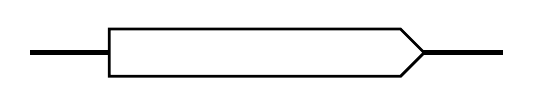
\begin{tikzpicture}

    % TikZ command: specify coordinates
    \coordinate (A)   at (0,0);
    \coordinate (B)   at (6,0);
    \coordinate (T)   at (5,0);

    % draw a track
    \maintrack (A) -- (B);

    % place a train on the track
    \train[forward] at (T) label ();

  \end{tikzpicture}
\end{document}
